\documentclass[../differential_methods.tex]{subfiles}
\begin{document}
\section{Aula 13 - 20 de Maio, 2026}
\subsection{Motivações}
\begin{itemize}
	\item Equação do Calor/de Difusão.
\end{itemize}
\subsection{Equação do Calor: método progressivo, retrógrado e Crank-Nickolson.}
Vamos considerar a equação do calor em um domínio limitado \(x\in (0, 1)\) para tempo \(t > t_{0} = 0\), um exemplo clássico da equação parabólica:
\[
	u_{t} = ku_{xx}, \quad 0<x<1,\; t>0.
\]
Precisamos de uma condição inicial em \(t_{0}=0\), como
\[
	u(x, 0) = \eta (x),\quad 0\leq x\leq 1
\]
e condições de contorno
\begin{align*}
	 & u(0, t) = g_{0}(t),\quad t>0   \\
	 & u(1, t) = g_{1}(t), \quad t>0.
\end{align*}
Para simplificar, vamos pedir que \(k=1\); caso k fosse negativo, \(u_{t}=ku_{xx}\) seria um problema de calor retrógrado, que é mal posto.

Para a discretização do domínio, considere uma grade discreta com pontos \((x_{i}, t_{n})\), onde
\[
	x_{i}=ih,\; t_{n}=nk,
\]
pois nesse ponto, já temos um certo conhecimento que podemos aplicar sobre discretização de problemas. Aqui, \(h=\Delta x\) é um distanciamento de malha no eixo x e \(k=\Delta t\) é um intervalo de tempo.

Tome \(U_{i}^{n}\approx u(x_{i}, t_{n})\) representando uma aproximação numérica de u em \((x_{i}, t_{n})\); uma bem natural seria utilizar a diferença progressiva
\begin{align*}
	\frac{u(x_{j}, t_{n}+\Delta t)-u(x_{j}, t_{n})}{\Delta t}+ \mathcal{O}(\Delta t) & = \frac{u(x_{j}+h, t_{n})-2u(x_{j}, t_{n}) + u(x_{j} -h, t_{n})}{h^{2}}+\mathcal{O}(h^{2})    \\
	\Rightarrow                                                                      & \frac{U_{i}^{n+1}-U_{i}^{n}}{\Delta t} = \frac{1}{h^{2}}(U_{i-1}^{n}-2U_{i}^{n}+U_{i+1}^{n}),
\end{align*}
que faz uso das já conhecidas diferenças centradas no espaço e uma diferença posterior de tempo. Como podemos computar cada \(U_{i}^{n+1}\) explicitamente em termos dos valores anteriores, este método é explícito:
\[
	\boxed{U_{i}^{n+1} = U_{i}^{n} + \frac{k}{h^{2}}(U_{i-1}^{n}-2U_{i}^{n}+U_{i+1}^{n})}
\]
Como já sabemos as condições iniciais e as de contorno, podemos começar a computar num ponto próximo da borda e, a partir dele, encontrar uma solução aproximada com isso, e é este o princípio geral do diferenças progressivas, conhecido também como \textit{método de Euler progressivo} (De novo!), utilizando um método de um passo temporalmente, conhecido como método de dois níveis, já que envolve a solução em dois tempos diferentes.

\begin{figure}[H]
	\begin{center}
		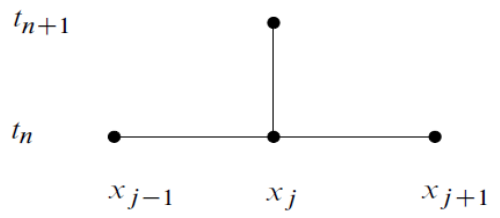
\includegraphics[height=\textheight, width=\textwidth, keepaspectratio]{./Images/border_13.png}
	\end{center}
\end{figure}

O método de diferenças progressivas pode ser representado matricialmente por
\begin{align*}
	\begin{bmatrix}
		U_{1}^{n+1}   \\
		U_{2}^{n+1}   \\
		U_{3}^{n+1}   \\
		\vdots        \\
		U_{m-1}^{n+1} \\
		U_{m}^{n+1}   \\
	\end{bmatrix} & = \begin{bmatrix}
		                  (1-2\sigma ) & \sigma       &              &        &        &              &              \\
		                  \sigma       & (1-2\sigma ) & \sigma       &        &        &              &              \\
		                               & \sigma       & (1-2\sigma ) & \sigma &        &              &              \\
		                               &              & \ddots       & \ddots & \ddots &              &              \\
		                               &              &              &        & \sigma & (1-2\sigma ) & \sigma       \\
		                               &              &              &        &        & \sigma       & (1-2\sigma )
	                  \end{bmatrix}\begin{bmatrix}
		                               U_{1}^{n}   \\
		                               U_{2}^{n}   \\
		                               U_{3}^{n}   \\
		                               \vdots      \\
		                               U_{m-1}^{n} \\
		                               U_{m}^{n}   \\
	                               \end{bmatrix}+ \\
	                 & + \begin{bmatrix}
		                     \sigma  g_{0}(t_{n}) \\
		                     0                    \\
		                     0                    \\
		                     \vdots               \\
		                     0                    \\
		                     \sigma g_1(t_{n})
	                     \end{bmatrix}.
\end{align*},
que equivale, sem as condições de contorno e colocando \(\sigma  = \frac{\Delta t }{h^{2}}\), à equação
\[
	U_{j}^{n+1} = \sigma U_{j-1}^{n} + (1-2\sigma )U_{j}^{n} + \sigma U_{j+1}^{n},
\]
ou, juntando tudo, ao sistema
\[
	U_{}^{n+1} = A U^{n} + g^{n}.
\]

Veremos mais alguns métodos hoje, incluindo o método regressivo e o método de \textit{Crank-Nickolson}

E se mudássemos a discretização? Agora, queremos uma discretização espacial, mas regressiva temporalmente, para a qual fica parecida com a progressiva, mas com uma mudança:
\begin{align*}
	\frac{u(x_{j}, t_{n})-u(x_{j}, t_{n}-\Delta  t)}{\Delta  t}+ \mathcal{O}(\Delta t) & = \frac{u(x_{j}+h, t_{n})-2u(x_{j}, t_{n}) + u(x_{j} -h, t_{n})}{h^{2}}+\mathcal{O}(h^{2}) \\
	\Rightarrow                                                                        & \frac{U_{j}^{n}-U_{j}^{n-1}}{\Delta t} = \frac{U_{j+1}^{n}-2U_{j}^{n}+U_{j+1}^{n}}{h^{2}},
\end{align*}
resultando no método
\[
	\boxed{\sigma U_{j-1}^{n+1} + (1+2\sigma )U_{j}^{n+1}-\sigma U_{j+1}^{n+1} = U_{j}^{n}}
\]
conhecido como \textit{Euler Regressivo} (Mais uma vez), que é o método de Euler implícito! Afinal, o estêncil desse método depende de pontos que dependem dos anteriores, resultando no sistema linear
\begin{align*}
	 & \begin{bmatrix}
		   (1-2\sigma ) & \sigma       &              &        &        &              &              \\
		   \sigma       & (1-2\sigma ) & \sigma       &        &        &              &              \\
		                & \sigma       & (1-2\sigma ) & \sigma &        &              &              \\
		                &              & \ddots       & \ddots & \ddots &              &              \\
		                &              &              &        & \sigma & (1-2\sigma ) & \sigma       \\
		                &              &              &        &        & \sigma       & (1-2\sigma )
	   \end{bmatrix}\begin{bmatrix}
		                U_{1}^{n+1}   \\
		                U_{2}^{n+1}   \\
		                U_{3}^{n+1}   \\
		                \vdots        \\
		                U_{m-1}^{n+1} \\
		                U_{m}^{n+1}   \\
	                \end{bmatrix} = \\
	 & =\begin{bmatrix}
		    U_{1}^{n}   \\
		    U_{2}^{n}   \\
		    U_{3}^{n}   \\
		    \vdots      \\
		    U_{m-1}^{n} \\
		    U_{m}^{n}   \\
	    \end{bmatrix} + \begin{bmatrix}
		                    \sigma  g_{0}(t_{n+1}) \\
		                    0                      \\
		                    0                      \\
		                    \vdots                 \\
		                    0                      \\
		                    \sigma g_1(t_{n+1})
	                    \end{bmatrix}
\end{align*}
O método ficou mais caro, mas veremos que ele tem uma vantagem em breve. Esperamos que esses métodos tenham erros de truncamento da ordem \(\mathcal{O}(\Delta t + h^{2})\), pois foram os dois termos descartados, e deseja-se que este erro tenda a zero quando \(\Delta t\) e h tendem a 0.

Quanto ao método de Crank-Nickolson, ele seria um método de diferenças centrais com uma maracutaia -- se fizermos um método por diferenças centrais usuais, gostaríamos de evitar fazer dois níveis por enquanto por conta da quantidade de pontos que ele vai envolver; faremos uma ampliação da malha espaço-temporal com \(t_{n+1/2} = t_{n} + \frac{\Delta t}{2}\), dando
\begin{align*}
	u(x_{n}, t_{n+1/2}) = u_{xx}(x_{j}, t_{n+1/2})                                            & = \frac{u(x_{n}, t_{n} + \Delta t) - u(x_{j}, t_{n})}{2\bigl(\frac{\Delta t}{2}\bigr)} + \mathcal{O}(\Delta t^{2}) \Rightarrow \\
	\frac{u(x_{n}, t_{n} + \Delta t) - u(x_{j}, t_{n})}{\Delta t} + \mathcal{O}(\Delta t^{2}) & = \frac{u(x_{j}-h, t_{n+1/2})-2u(x_{j}, t_{n+1/2})+u(x_{j}+h, t_{n+1/2})}{h^{2}}                                               \\
	                                                                                          & +\mathcal{O}(h^{2}),
\end{align*}
só que isso resulta em pontos no meio da malha, e isso aumenta a resolução do problema mais do que deveria, criando graus de liberdade a mais. Como resolver isso? Interpolando na média! Daí, o lado direito ganha um erro de interpolação e fica
\begin{align*}
	\frac{1}{2h^{2}} & \biggl(u(x_{j}-h, t_{n+1})-2u(x_{j}, t_{n+1})+u(x_{j}+h, t_{n+1})                              \\
	                 & + u(x_{j}-h, t_{n})-2u(x_{j}, t_{n}) + u(x_{j}+h, t_{n})\biggr)+\mathcal{O}(h^{2})+\varepsilon
\end{align*}
Passando a discretização, obtemos
\begin{align*}
	            & \frac{U_{j}^{n+1}-U_{i}^{n}}{\Delta t} = \frac{1}{2}\frac{U_{j-1}^{n+1}-2U_{j}^{n}+U_{j+1}^{n+1}}{h^{2}} + \frac{1}{2}\frac{U_{j-1}^{n}-2U_{j}^{n}+U_{j+1}^{n}}{h^{2}}   \\
	\Rightarrow & U_{j}^{n+1}-U_{j}^{n}=\frac{\sigma }{2} (U_{j+1}^{n+1}-2U_{j}^{n+1}+U_{j+1}^{n+1}+\frac{\sigma }{2} (U_{j-1}^{n}-2U_{j}^{n}+U_{j+1}^{n})                                 \\
	\Rightarrow & -\frac{\sigma }{2}U_{j}^{n+1} + (1+\sigma )U_{j}^{n+1} -\frac{\sigma }{2}U_{j+1}^{n+1} = \frac{\sigma }{2}U_{j-1}^{n}+(1-\sigma )U_{j}^{n}+\frac{\sigma }{2}U_{j+1}^{n},
\end{align*}
cuja matriz fica
\begin{align*}
	  & \begin{bmatrix}
		    (1+\sigma )        & -\frac{\sigma }{2} &                    &                    &                    &                    &                    \\
		    -\frac{\sigma }{2} & (1+\sigma )        & -\frac{\sigma }{2} &                    &                    &                    &                    \\
		                       & -\frac{\sigma }{2} & (1+\sigma )        & -\frac{\sigma }{2} &                    &                    &                    \\
		                       &                    & \ddots             & \ddots             & \ddots             &                    &                    \\
		                       &                    &                    &                    & -\frac{\sigma }{2} & (1+\sigma )        & -\frac{\sigma }{2} \\
		                       &                    &                    &                    &                    & -\frac{\sigma }{2} & (1+\sigma )
	    \end{bmatrix}\begin{bmatrix}
		                 U_{1}^{n+1}   \\
		                 U_{2}^{n+1}   \\
		                 U_{3}^{n+1}   \\
		                 \vdots        \\
		                 U_{m-1}^{n+1} \\
		                 U_{m}^{n+1}   \\
	                 \end{bmatrix} = \\
	= & \begin{bmatrix}
		    (1-\sigma )       & \frac{\sigma }{2} &                   &                   &                   &                   &                   \\
		    \frac{\sigma }{2} & (1-\sigma )       & \frac{\sigma }{2} &                   &                   &                   &                   \\
		                      & \frac{\sigma }{2} & (1-\sigma )       & \frac{\sigma }{2} &                   &                   &                   \\
		                      &                   & \ddots            & \ddots            & \ddots            &                   &                   \\
		                      &                   &                   &                   & \frac{\sigma }{2} & (1-\sigma )       & \frac{\sigma }{2} \\
		                      &                   &                   &                   &                   & \frac{\sigma }{2} & (1-\sigma )
	    \end{bmatrix}\begin{bmatrix}
		                 U_{1}^{n}   \\
		                 U_{2}^{n}   \\
		                 U_{3}^{n}   \\
		                 \vdots      \\
		                 U_{m-1}^{n} \\
		                 U_{m}^{n}   \\
	                 \end{bmatrix}        \\
	  & + \begin{bmatrix}
		      \frac{\sigma }{2} (g_{0}(t_{n+1}+g_{0}(t_{n})) \\
		      0                                              \\
		      0                                              \\
		      \vdots                                         \\
		      0                                              \\
		      \frac{\sigma }{2} (g_{1}(t_{n+1}+g_{1}(t_{n}))
	      \end{bmatrix}
\end{align*}
No fim, é só muita conta algébrica mesmo. Este método ainda é um método implícito, afinal as incógnitas estão dependendo umas das outras, como dá para ver no sistema linear acima da forma
\[
	A\underline{U}^{n+1} = B\underline{U}^{n} + \underline{g}^{n} + \underline{g}^{n+1},
\]
resultando no método de Crank-Nickolson
\[
	\boxed{-\frac{\sigma }{2}U_{j}^{n+1} + (1+\sigma )U_{j}^{n+1} -\frac{\sigma }{2}U_{j+1}^{n+1} = \frac{\sigma }{2}U_{j-1}^{n}+(1-\sigma )U_{j}^{n}+\frac{\sigma }{2}U_{j+1}^{n}}
\]
\textbf{Não é potência! É índice!}

O problema é se essas aproximações que fizemos forem resultar numa redução da ordem do método. Para verificar isso, precisamos ver o erro de truncamento de cada um deles, ou seja, \(\tau_{F}(x_{i}, t_{n})\) do Euler-Forward, \(\tau_{B}(x_{i}, t_{n})\) pro Euler-Backward e \(\tau_{CN}(x_{i}, t_{n})\).
Neste sentido, a definição é a mesma de sempre, resultando em
\[
	\tau_{F}(x, t) = \frac{u(x, t+\Delta t) - u(x, t)}{\Delta t} - \frac{1}{h^{2}}(u(x-h, t) - 2u(x, t) + u(x+h, t)),
\]
onde devemos ter cuidado com usar a forma de diferenças que modelam diretamente a equação diferencial. Agora, é questão de expandir em Taylor.
\end{document}
